
\section{Sprint 1 Summary}

In sprint 1, the main focus has been planning and research, how the group is organized, requirements and test specification. This sprint has mostly been centered around providing the right documentation to HSN, as well as preparing the first oral presentation. The group had to establish a clear understanding of how to work in parallel to accomplish the build and integration of the quadcopters.
\newline \newline
During this sprint we got the first variable pitch mechanisms from Hobbyking in China. 

\begin{figure}[h]
        \centering
         \begin{minipage}[b]{0.4\textwidth}
            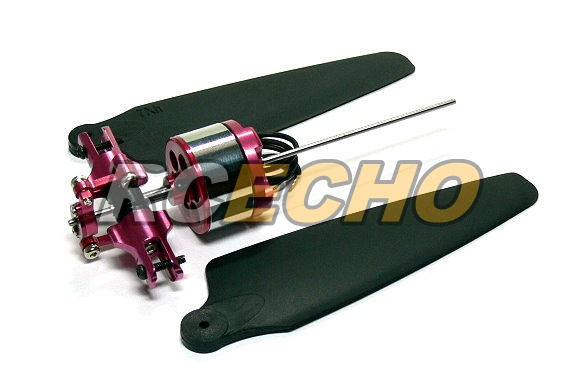
\includegraphics[width = 1\textwidth]{VAPIQ-PICTURES/VPitchAeoc20}
              \caption{AEO C20, variable pitch mechanism}
            \label{fig:testpic2}
        \end{minipage}
        \hfill
        \begin{minipage}[b]{0.4\textwidth}
            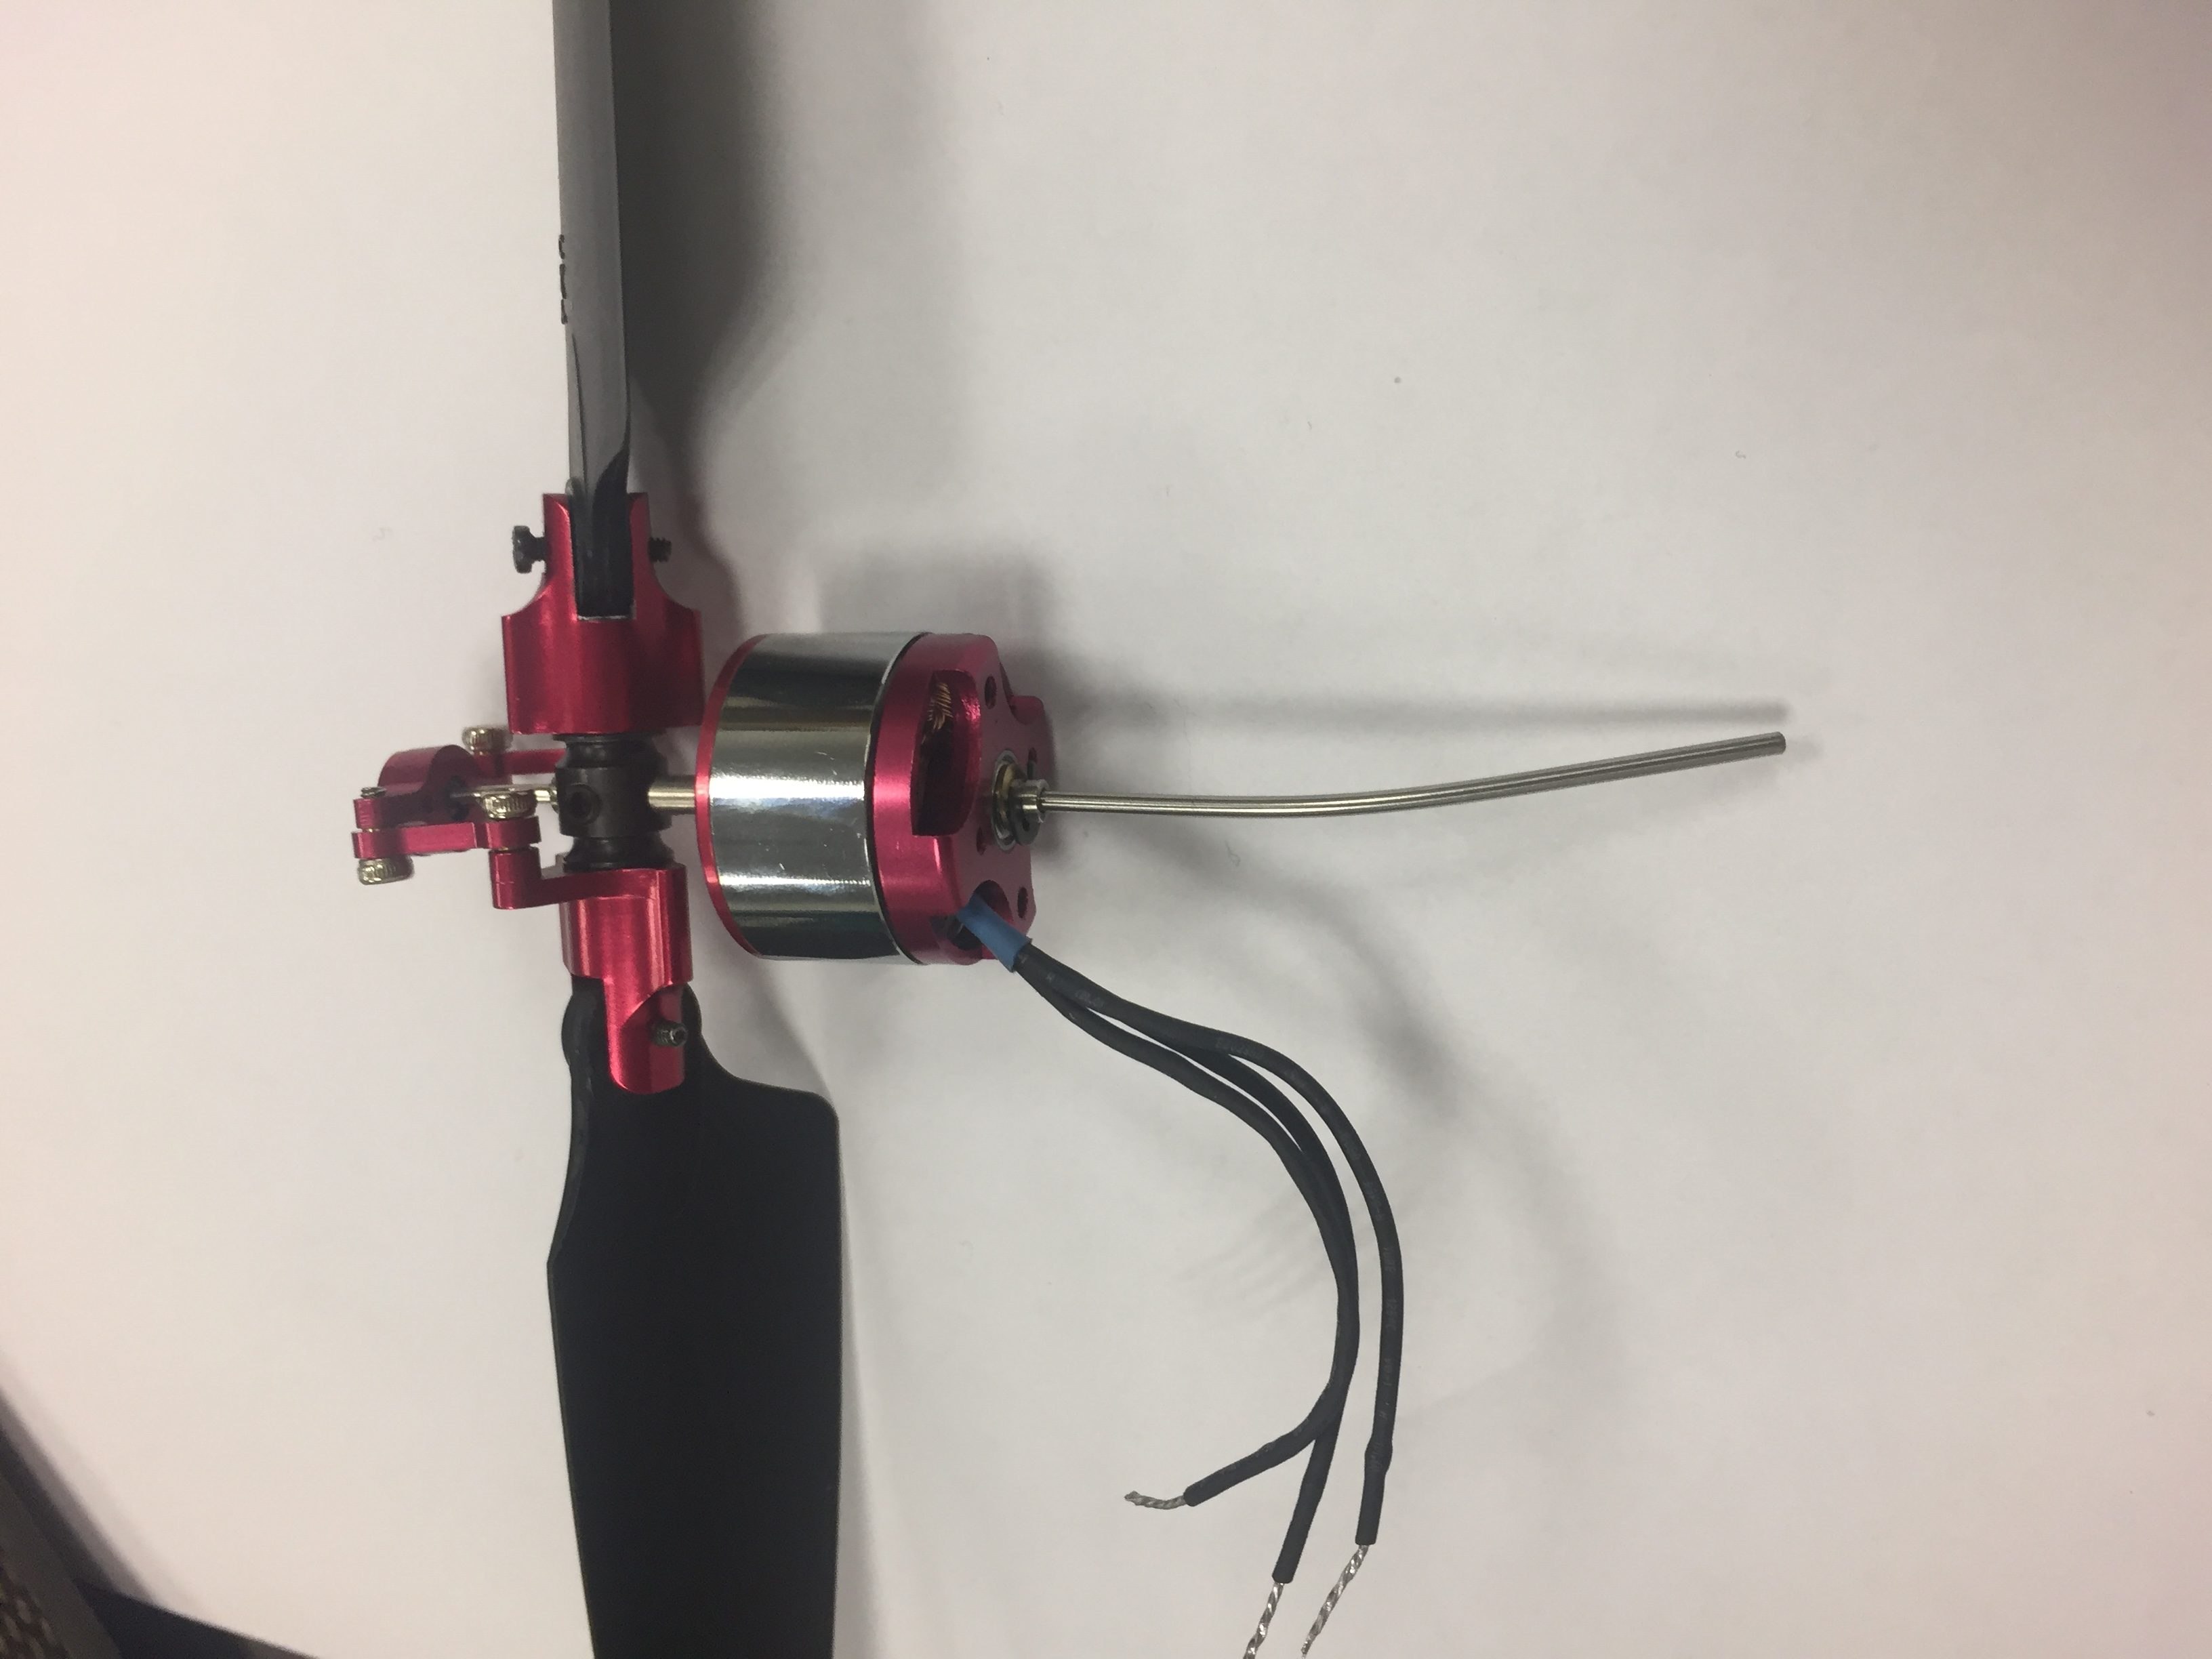
\includegraphics[width = 0.7\textwidth]{VAPIQ-PICTURES/File_004}
            \caption{Recived Item}
            \label{fig:testpic3}
        \end{minipage}
\end{figure}
\\
The mechanisms was of poor quality, and the shaft on every mechanism was severely bent and could not be used. By comparing the picture from Hobbyking and the one we got, we concluded that the mechanism was a fake and not an original part. The group did research on existing variable pitch mechanisms, but there are very few available. This made us consider the tail rotor mechanism of an Align T-rex helicopter. Most RC helicopter-tails have variable pitch, most often with belt drive. If we want to have four separate motors with RPM control as well, the helicopter tail mechanisms needs to be modified.
\\\\
Additionally in sprint 1, the group got familiar with the motion capture system Qualisys at KIC and have made a simulation of quadcopter dynamics in Python. Development of the project webpage has also started.

\subsection{Completion and Scope Change}

In sprint 1, all activities in the project plan was executed, 90 \% of all planned tasks where accomplished. Some technical tasks was postponed due to documentation and presentation 1. The remaining 10\% of tasks were reevaluated, and if needed brought into sprint 2. 
There was 5\% scope change, this was due to tasks not identified in the planning phase, concerning documentation.
The spike in the graph is due to a change in the way tasks and story points are rated and allocated in JIRA, and is not a real change in scope. 
\\

Projectplan status:

	Start-Up Phase:
	\begin{itemize}
	\item Research, Done
	\item Stakeholder Analysis, ?
	\item Documentation, Done
	\item Project Model, Done
	\item Project Plan V.1, Done
	\item Requirements V.1, Done
	\item Test Specification V.1, Done
	\item Document Templates, Done
	\item First Presentation, Done
	\item Presentation 1, Done
    \item Preliminary Documentation Refinement, Done
	\item Presentation Refinement, Done
	\item Presentation Practice, Done
	\end{itemize}
	
	Sprint 1:
	\begin{itemize}
	\item Control System Research, Done
    \item Preliminary Flight Simulation, Done
	\item Flight Controller Research, Done
	\item Mechanical Design Study, In progress 
	\item Communication With Qualisys, Not completed
	\item Start Developing Web Page, Done   
	\end{itemize}

\begin{figure}[h]
        \centering
        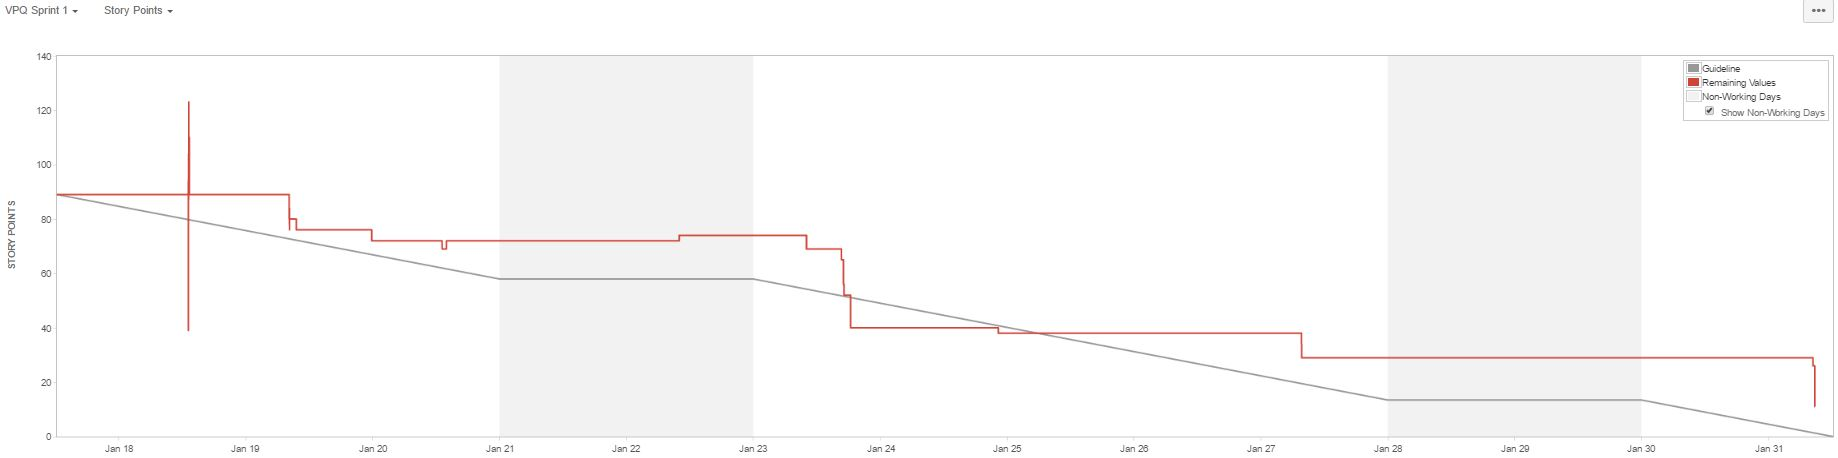
\includegraphics[width = 1\textwidth]{VAPIQ-PICTURES/BDSprint1}
        \caption{Sprint 1}
        %\\[2.0 cm]
    \end{figure}  

\subsection{Challenges}
%Mechanisms did not work, motors was destroyed, could not start the design without the right hardware. Lite penger har utsatt bygging. 


The biggest challenge encountered in sprint 1 was that the mechanisms we planned to use was of bad quality and we therefore had to reevaluate. Other challenges were time estimation and time-logging. We experienced that our estimates of time often were incorrect and had to make changes on how we planned each sprint.

\subsection{Results and Conclusions}

The documents produced in sprint 1:
\begin{itemize}
    \item Organizational Document, containing project
 plan and organization
    \item Backlog And Traceability Document
    \item Test Specification
    \item Qualisys Document
    \item Feasibility Study
    \item Project Model
\end{itemize}
\\\\
In sprint 2, the main focus will be on creating the first prototype. The critical activity for sprint 2 is to create a design, order
components, allowing flight controller experiments to be performed
in KIC.

%Comments?
\subsection{Lessons Learned}

The group got feedback that our motivation for the project was unclear in presentation 1. The group should also minimize the amount of documentation and be more selective of content. Consider making bigger documents instead of many separate ones.
The group also learned to be more sceptical of components from unknown vendors in China.


